\documentclass[aspectratio=169,11pt]{beamer}

\usetheme{Madrid}
\usecolortheme{default}
\setbeamertemplate{navigation symbols}{}
\setbeamertemplate{footline}[frame number]

\usepackage{amsmath,amssymb}
\usepackage{tikz}
\usetikzlibrary{positioning,calc}

\definecolor{RamRed}{RGB}{190,40,45}
\definecolor{RamBlue}{RGB}{30,90,180}
\definecolor{SoftGray}{RGB}{245,245,245}
\definecolor{DarkGray}{RGB}{70,70,70}

\setbeamercolor{title}{fg=DarkGray}
\setbeamercolor{frametitle}{fg=white,bg=RamBlue}
\setbeamercolor{structure}{fg=RamBlue}

\tikzset{
  v/.style={circle,draw=black,fill=white,inner sep=1.8pt},
  rededge/.style={draw=RamRed,line width=1.25pt},
  blueedge/.style={draw=RamBlue,line width=1.25pt},
  grayedge/.style={draw=black!35,line width=0.7pt},
  topic/.style={draw=black!30,fill=SoftGray,rounded corners=5pt,inner sep=7pt,
    text width=5.8cm,minimum height=1.65cm,align=left},
}

\newcommand{\Ram}{\operatorname{R}}

\title[Ramsey Numbers]{Ramsey Numbers}
\subtitle{Section 1.8 of Harris--Hirst--Mossinghoff}
\author{Combinatorics and Graph Theory}
\date{}

\begin{document}

\begin{frame}[plain]
  \centering
  \vspace{0.4cm}
  {\Huge\bfseries Ramsey Numbers}\par
  \vspace{0.25cm}
  {\Large Section 1.8}\par
  \vspace{0.15cm}
  {\large Harris--Hirst--Mossinghoff, \emph{Combinatorics and Graph Theory}}\par

  \vspace{0.9cm}
  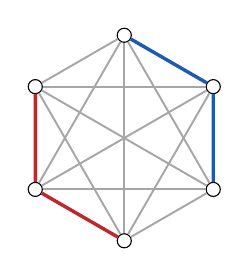
\begin{tikzpicture}[scale=0.9]
    \foreach \i in {1,...,6} {\node[v] (a\i) at ({90+60*\i}:1.45) {};}
    \foreach \i/\j in {1/2,2/3,3/4,4/5,5/6,6/1,1/3,1/5,2/4,2/6,3/5,4/6,1/4,2/5,3/6} {\draw[grayedge] (a\i)--(a\j);}
    \draw[rededge] (a1)--(a2)--(a3)--cycle;
    \draw[blueedge] (a4)--(a5)--(a6)--cycle;
  \end{tikzpicture}

\end{frame}

\begin{frame}[plain]
\centering
\vspace{0.15cm}
{\Huge\bfseries Today's lecture}\par
\vspace{0.55cm}

\large
\begin{columns}[T,onlytextwidth]
  \begin{column}{0.48\textwidth}
    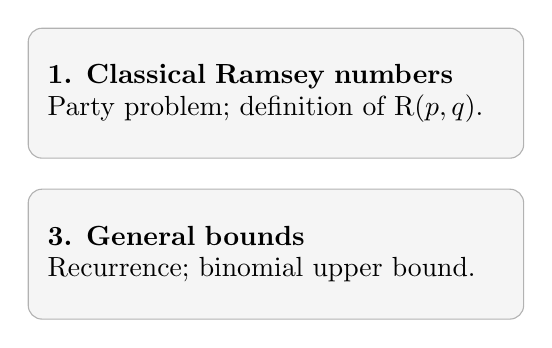
\begin{tikzpicture}
      \node[topic] (a) {\textbf{1. Classical Ramsey numbers}\\[-0.02cm]
      Party problem; definition of $\Ram(p,q)$.};
      \node[topic,below=0.38cm of a] (c) {\textbf{3. General bounds}\\[-0.02cm]
      Recurrence; binomial upper bound.};
    \end{tikzpicture}
  \end{column}
  \begin{column}{0.48\textwidth}
    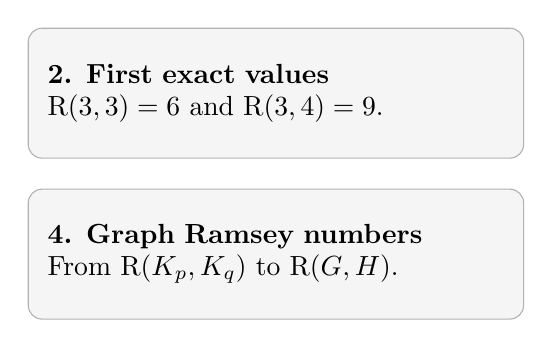
\begin{tikzpicture}
      \node[topic] (b) {\textbf{2. First exact values}\\[-0.02cm]
      $\Ram(3,3)=6$ and $\Ram(3,4)=9$.};
      \node[topic,below=0.38cm of b] (d) {\textbf{4. Graph Ramsey numbers}\\[-0.02cm]
      From $\Ram(K_p,K_q)$ to $\Ram(G,H)$.};
    \end{tikzpicture}
  \end{column}
\end{columns}
\end{frame}

\section{Motivating Question}

\begin{frame}{The party problem}
\large

You are going to a party. Some pairs of people already know each other,
and some pairs of people are strangers.

\vspace{0.45cm}

Assume that for every pair of people, exactly one of these two possibilities holds:

\vspace{0.35cm}

\begin{center}
  \begin{columns}[c,onlytextwidth]
    \begin{column}{0.43\textwidth}
      \begin{block}{}
        \centering
        they know each other
      \end{block}
    \end{column}
    \begin{column}{0.10\textwidth}
      \centering or
    \end{column}
    \begin{column}{0.43\textwidth}
      \begin{block}{}
        \centering
        they are strangers
      \end{block}
    \end{column}
  \end{columns}
\end{center}

\vspace{0.35cm}

\begin{alertblock}{Question}
  \centering
  How many people are needed to guarantee either\\[0.08cm]
  \textbf{three mutual acquaintances} or \textbf{three mutual strangers}?
\end{alertblock}
\end{frame}

\begin{frame}{The party problem as an edge-colouring problem}
\large

\begin{columns}[T,onlytextwidth]
  \begin{column}{0.46\textwidth}
    \begin{block}{Build the complete graph $K_n$}
      \begin{itemize}
        \item each person is a vertex;
        \item each pair of people is joined by an edge.
      \end{itemize}
    \end{block}
  \end{column}
  \begin{column}{0.46\textwidth}
    \begin{block}{Colour every edge}
      \begin{itemize}
        \item \textcolor{RamRed}{red}: the two people know each other;
        \item \textcolor{RamBlue}{blue}: the two people are strangers.
      \end{itemize}
    \end{block}
  \end{column}
\end{columns}

\vspace{0.22cm}

\begin{alertblock}{Equivalent question}
  \centering
  How large must $n$ be so that every red--blue edge-colouring of $K_n$
  contains a \textbf{monochromatic} copy of $K_3$?
\end{alertblock}

\vspace{0.08cm}

\begin{center}
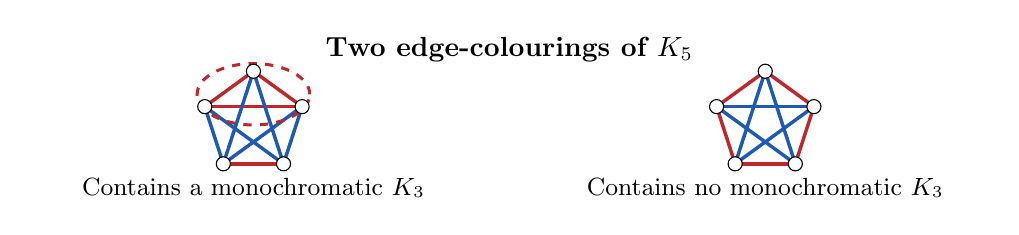
\begin{tikzpicture}[font=\small]
  \node[font=\bfseries] at (0,0.93) {Two edge-colourings of $K_5$};

  % Left: a colouring containing a red triangle.
  \begin{scope}[xshift=-3.25cm,scale=0.65]
    \foreach \i/\angle in {1/90,2/162,3/234,4/306,5/18}
      \coordinate (l\i) at (\angle:1.0);

    \foreach \i/\j in {1/2,1/5,2/5,3/4}
      \draw[rededge] (l\i)--(l\j);
    \foreach \i/\j in {1/3,1/4,2/3,2/4,3/5,4/5}
      \draw[blueedge] (l\i)--(l\j);

    \draw[RamRed,dashed,line width=1.1pt] (0,0.55) ellipse (1.10 and 0.60);
    \foreach \i in {1,...,5} \node[v] at (l\i) {};
  \end{scope}
  \node[align=center,text width=5.5cm] at (-3.25,-0.83)
    {Contains a monochromatic $K_3$};

  % Right: each colour class is a 5-cycle, so there is no triangle.
  \begin{scope}[xshift=3.25cm,scale=0.65]
    \foreach \i/\angle in {1/90,2/162,3/234,4/306,5/18}
      \coordinate (r\i) at (\angle:1.0);

    \foreach \i/\j in {1/2,2/3,3/4,4/5,5/1}
      \draw[rededge] (r\i)--(r\j);
    \foreach \i/\j in {1/3,1/4,2/4,2/5,3/5}
      \draw[blueedge] (r\i)--(r\j);

    \foreach \i in {1,...,5} \node[v] at (r\i) {};
  \end{scope}
  \node[align=center,text width=5.5cm] at (3.25,-0.83)
    {Contains no monochromatic $K_3$};
\end{tikzpicture}
\end{center}
\end{frame}

\section{Classical Ramsey Numbers}

\begin{frame}{Now, some definitions}
\large

\begin{block}{2-colouring}
  A \textbf{2-colouring} of the edges of a graph assigns one of two colours
  to every edge.
\end{block}

\vspace{0.35cm}

\begin{alertblock}{Classical Ramsey number}
  Let $p$ and $q$ be positive integers. The \textbf{Ramsey number}
  $\Ram(p,q)$ is the smallest integer $n$ such that every 2-colouring of the
  edges of $K_n$ contains either
  \[
    \text{a red }K_p
    \qquad\text{or}\qquad
    \text{a blue }K_q
  \]
  as a subgraph.
\end{alertblock}

\vspace{0.35cm}

\begin{center}
  In particular, $\Ram(3,3)$ answers the party problem.
\end{center}
\end{frame}

\begin{frame}[t]{Basic Question}
\vspace{0.10cm}

\begin{block}{Question}
\large
Suppose $n>\Ram(p,q)$. Then every 2-colouring of the edges of $K_n$
must contain either \textcolor{RamRed}{a red $K_p$} or
\textcolor{RamBlue}{a blue $K_q$}. Why?
\end{block}
\end{frame}

\begin{frame}[t]{Basic Question}
\vspace{0.10cm}

\begin{block}{Question}
\large
Suppose $n>\Ram(p,q)$. Then every 2-colouring of the edges of $K_n$
must contain either \textcolor{RamRed}{a red $K_p$} or
\textcolor{RamBlue}{a blue $K_q$}. Why?
\end{block}

\vspace{0.30cm}

\begin{alertblock}{Answer}
\large
Removing $m$ vertices from $K_n$ leaves the complete graph $K_{n-m}$.
Take
\[
  m=n-\Ram(p,q).
\]
The remaining vertices span a copy of $K_{\Ram(p,q)}$. Any 2-colouring
of $K_n$ restricts to a 2-colouring of this subgraph, which contains a
\textcolor{RamRed}{red $K_p$} or a \textcolor{RamBlue}{blue $K_q$} by
the definition of $\Ram(p,q)$.
\end{alertblock}
\end{frame}

\begin{frame}[t]{Next Question}
\vspace{0.10cm}

\begin{block}{Question}
\large
What is the value of $\Ram(1,3)$?
\end{block}
\end{frame}

\begin{frame}[t]{Next Question}
\vspace{0.10cm}

\begin{block}{Question}
\large
What is the value of $\Ram(1,3)$?
\end{block}

\vspace{0.35cm}

\begin{alertblock}{Answer}
\large
\[
  \boxed{\Ram(1,3)=1}.
\]
The graph $K_1$ has one vertex and no edges. Thus, in every 2-colouring
of $K_1$, the single vertex already forms a red $K_1$: there are no edges
that could fail to be red.

\vspace{0.25cm}

Therefore $n=1$ satisfies the definition, and it is the smallest possible
positive integer.
\end{alertblock}

\vfill

\begin{block}{Follow-Up Question}
\large
What about the value of $\Ram(1,k)$?
\end{block}
\end{frame}

\begin{frame}[t]{Next Question}
\vspace{0.10cm}

\begin{block}{Question}
\large
What is the value of $\Ram(2,4)$?
\end{block}
\end{frame}

\begin{frame}[t]{Next Question}
\vspace{0.10cm}

\begin{block}{Question}
\large
What is the value of $\Ram(2,4)$?
\end{block}

\vspace{0.30cm}

\begin{alertblock}{Claim}
\large
\[
  \boxed{\Ram(2,4)=4}.
\]
We will prove this claim in two steps.

\vspace{0.18cm}

\textbf{Step 1.}
Show that $\Ram(2,4)>3$ by exhibiting a 2-colouring of $K_3$
with no red $K_2$ and, trivially, no blue $K_4$.

\vspace{0.18cm}

\textbf{Step 2.}
Show that $\Ram(2,4)\le 4$ by proving that every 2-colouring of
$K_4$ contains a red $K_2$ or a blue $K_4$.
\end{alertblock}
\end{frame}

\begin{frame}[t]{Showing $\Ram(2,4)>3$}
\vspace{0.05cm}

\begin{center}
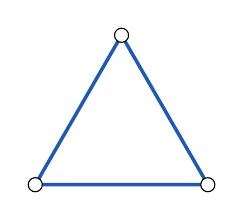
\begin{tikzpicture}[scale=1.10]
  \coordinate (a) at (90:1.15);
  \coordinate (b) at (210:1.15);
  \coordinate (c) at (330:1.15);
  \draw[blueedge] (a)--(b)--(c)--cycle;
  \foreach \p in {a,b,c} \node[v] at (\p) {};
\end{tikzpicture}
\end{center}

\begin{block}{Why this colouring works}
\large
Every edge is \textcolor{RamBlue}{blue}, so there is no
\textcolor{RamRed}{red $K_2$}.

\vspace{0.18cm}

The graph has only three vertices, so it cannot contain a
\textcolor{RamBlue}{blue $K_4$}.
\end{block}

\begin{alertblock}{Conclusion}
\large
Thus, $\Ram(2,4)>3$.
\end{alertblock}
\end{frame}

\begin{frame}[t]{Showing $\Ram(2,4)\le 4$}
\vspace{0.10cm}

\begin{block}{Proof}
\large
Consider any 2-colouring of the edges of $K_4$. There are two cases.
\end{block}

\vspace{0.10cm}

\begin{columns}[T,onlytextwidth]
  \begin{column}{0.48\textwidth}
    \begin{block}{Case 1: a red edge occurs}
      \centering
      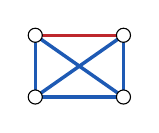
\begin{tikzpicture}[scale=0.56]
        \coordinate (a) at (-1,0.7);
        \coordinate (b) at (1,0.7);
        \coordinate (c) at (-1,-0.7);
        \coordinate (d) at (1,-0.7);
        \draw[rededge] (a)--(b);
        \foreach \x/\y in {a/c,a/d,b/c,b/d,c/d}
          \draw[blueedge] (\x)--(\y);
        \foreach \p in {a,b,c,d} \node[v] at (\p) {};
      \end{tikzpicture}

      \vspace{0.04cm}
      \textcolor{RamRed}{That edge is a red $K_2$.}
    \end{block}
  \end{column}
  \begin{column}{0.48\textwidth}
    \begin{block}{Case 2: no red edge occurs}
      \centering
      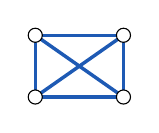
\begin{tikzpicture}[scale=0.56]
        \coordinate (a) at (-1,0.7);
        \coordinate (b) at (1,0.7);
        \coordinate (c) at (-1,-0.7);
        \coordinate (d) at (1,-0.7);
        \foreach \x/\y in {a/b,a/c,a/d,b/c,b/d,c/d}
          \draw[blueedge] (\x)--(\y);
        \foreach \p in {a,b,c,d} \node[v] at (\p) {};
      \end{tikzpicture}

      \vspace{0.04cm}
      \textcolor{RamBlue}{The whole graph is a blue $K_4$.}
    \end{block}
  \end{column}
\end{columns}

\vspace{0.12cm}

\begin{alertblock}{Conclusion}
\large
Every 2-colouring of $K_4$ contains a red $K_2$ or a blue $K_4$.
Therefore, $\Ram(2,4)\le 4$.
\end{alertblock}
\end{frame}

\begin{frame}[t]{Follow-Up Question}
\vspace{0.10cm}

\begin{block}{Question}
\large
What about the value of $\Ram(2,n)$?
\end{block}
\end{frame}

\begin{frame}[t]{The value of $\Ram(2,n)$}
\vspace{0.10cm}

\begin{block}{Question}
\large
What about the value of $\Ram(2,n)$?
\end{block}

\vspace{0.25cm}

\begin{alertblock}{Claim}
\large
\[
  \boxed{\Ram(2,n)=n}.
\]
\end{alertblock}

\begin{block}{The same argument gives both bounds}
\large
For $\Ram(2,n)>n-1$, colour every edge of $K_{n-1}$
\textcolor{RamBlue}{blue}. There is no \textcolor{RamRed}{red $K_2$}, and
there are too few vertices for a \textcolor{RamBlue}{blue $K_n$}.

\vspace{0.25cm}

For $\Ram(2,n)\le n$, consider any 2-colouring of $K_n$. A
\textcolor{RamRed}{red edge} gives a red $K_2$; if there is no red edge, then
all edges are \textcolor{RamBlue}{blue}, giving a blue $K_n$.
\end{block}
\end{frame}

\begin{frame}[t]{Computing Another Ramsey Number}
\vspace{0.10cm}

\begin{alertblock}{Claim}
\large
\[
  \boxed{\Ram(3,3)=6}.
\]
\end{alertblock}

\vspace{0.22cm}

\begin{block}{Proof}
\large
Again, we will prove the claim in two steps.

\vspace{0.20cm}

\textbf{Step 1.}
Show that $\Ram(3,3)>5$ by exhibiting a 2-colouring of $K_5$ with
neither a \textcolor{RamRed}{red $K_3$} nor a \textcolor{RamBlue}{blue $K_3$}.

\vspace{0.22cm}

\textbf{Step 2.}
Show that $\Ram(3,3)\le 6$ by proving that every 2-colouring of $K_6$
contains a \textcolor{RamRed}{red $K_3$} or a \textcolor{RamBlue}{blue $K_3$}.
\end{block}
\end{frame}

\begin{frame}[t]{Showing $\Ram(3,3)>5$}
\vspace{0.05cm}

\begin{center}
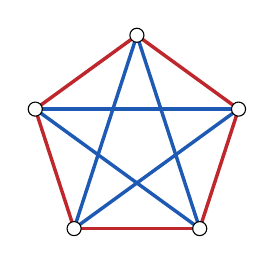
\begin{tikzpicture}[scale=1.15]
  \foreach \i/\angle in {1/90,2/162,3/234,4/306,5/18}
    \coordinate (v\i) at (\angle:1.18);

  \foreach \i/\j in {1/2,2/3,3/4,4/5,5/1}
    \draw[rededge] (v\i)--(v\j);
  \foreach \i/\j in {1/3,1/4,2/4,2/5,3/5}
    \draw[blueedge] (v\i)--(v\j);
  \foreach \i in {1,...,5} \node[v] at (v\i) {};
\end{tikzpicture}
\end{center}

\begin{block}{Why this colouring works}
\large
Notice that this 2-colouring of $K_5$ contains no
\textcolor{RamRed}{red} or \textcolor{RamBlue}{blue} $K_3$ subgraph.

\vspace{0.20cm}

Therefore, $\Ram(3,3)>5$.
\end{block}
\end{frame}

\begin{frame}[t]{Showing $\Ram(3,3)\le 6$}
\vspace{0.05cm}

\begin{center}
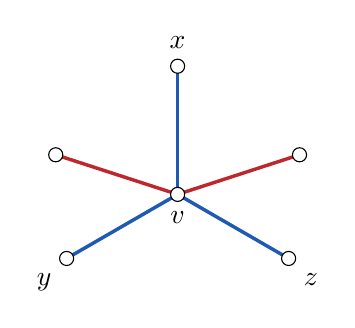
\begin{tikzpicture}[scale=1.05]
  \coordinate (v0) at (0,0);
  \coordinate (x) at (90:1.55);
  \coordinate (y) at (210:1.55);
  \coordinate (z) at (330:1.55);
  \coordinate (r1) at (162:1.55);
  \coordinate (r2) at (18:1.55);

  \draw[blueedge] (v0)--(x);
  \draw[blueedge] (v0)--(y);
  \draw[blueedge] (v0)--(z);
  \draw[rededge] (v0)--(r1);
  \draw[rededge] (v0)--(r2);

  \node[v,label=below:$v$] at (v0) {};
  \node[v,label=above:$x$] at (x) {};
  \node[v,label=below left:$y$] at (y) {};
  \node[v,label=below right:$z$] at (z) {};
  \node[v] at (r1) {};
  \node[v] at (r2) {};
\end{tikzpicture}
\end{center}

\begin{block}{The pigeonhole idea}
\large
Choose any vertex $v$ of $K_6$. Its five incident edges are coloured red or
blue, so at least three have the same colour.

\vspace{0.20cm}

Without loss of generality, suppose $v$ is joined to $x,y,z$ by
\textcolor{RamBlue}{blue} edges.
\end{block}
\end{frame}

\begin{frame}[t]{Showing $\Ram(3,3)\le 6$}
\vspace{0.05cm}

\begin{block}{What happens among $x,y,z$?}
\large
Recall that $vx$, $vy$, and $vz$ are \textcolor{RamBlue}{blue}. There are two cases.
\end{block}

\vspace{0.10cm}

\begin{columns}[T,onlytextwidth]
  \begin{column}{0.48\textwidth}
    \begin{block}{Case 1: a blue edge occurs}
      \centering
      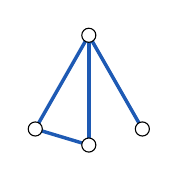
\begin{tikzpicture}[scale=0.68]
        \coordinate (v0) at (0,1.20);
        \coordinate (x) at (-1.0,-0.55);
        \coordinate (y) at (0,-0.85);
        \coordinate (z) at (1.0,-0.55);
        \draw[blueedge] (v0)--(x);
        \draw[blueedge] (v0)--(y);
        \draw[blueedge] (v0)--(z);
        \draw[blueedge] (x)--(y);
        \foreach \p in {v0,x,y,z} \node[v] at (\p) {};
      \end{tikzpicture}

      \textcolor{RamBlue}{The edge $xy$ closes a blue $K_3$.}
    \end{block}
  \end{column}
  \begin{column}{0.48\textwidth}
    \begin{block}{Case 2: no blue edge occurs}
      \centering
      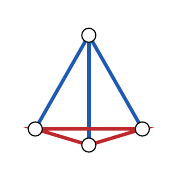
\begin{tikzpicture}[scale=0.68]
        \coordinate (v0) at (0,1.20);
        \coordinate (x) at (-1.0,-0.55);
        \coordinate (y) at (0,-0.85);
        \coordinate (z) at (1.0,-0.55);
        \draw[blueedge] (v0)--(x);
        \draw[blueedge] (v0)--(y);
        \draw[blueedge] (v0)--(z);
        \draw[rededge] (x)--(y)--(z)--cycle;
        \foreach \p in {v0,x,y,z} \node[v] at (\p) {};
      \end{tikzpicture}

      \textcolor{RamRed}{Then $xyz$ is a red $K_3$.}
    \end{block}
  \end{column}
\end{columns}

\vspace{0.10cm}

\begin{alertblock}{Conclusion}
\large
Every 2-colouring of $K_6$ contains a red or blue $K_3$. Thus,
$\Ram(3,3)\le 6$.
\end{alertblock}
\end{frame}

\end{document}
